\documentclass[twoside]{book}

% Packages required by doxygen
\usepackage{fixltx2e}
\usepackage{calc}
\usepackage{doxygen}
\usepackage[export]{adjustbox} % also loads graphicx
\usepackage{graphicx}
\usepackage[utf8]{inputenc}
\usepackage{makeidx}
\usepackage{multicol}
\usepackage{multirow}
\PassOptionsToPackage{warn}{textcomp}
\usepackage{textcomp}
\usepackage[nointegrals]{wasysym}
\usepackage[table]{xcolor}

% Font selection
\usepackage[T1]{fontenc}
\usepackage[scaled=.90]{helvet}
\usepackage{courier}
\usepackage{amssymb}
\usepackage{sectsty}
\renewcommand{\familydefault}{\sfdefault}
\allsectionsfont{%
  \fontseries{bc}\selectfont%
  \color{darkgray}%
}
\renewcommand{\DoxyLabelFont}{%
  \fontseries{bc}\selectfont%
  \color{darkgray}%
}
\newcommand{\+}{\discretionary{\mbox{\scriptsize$\hookleftarrow$}}{}{}}

% Page & text layout
\usepackage{geometry}
\geometry{%
  a4paper,%
  top=2.5cm,%
  bottom=2.5cm,%
  left=2.5cm,%
  right=2.5cm%
}
\tolerance=750
\hfuzz=15pt
\hbadness=750
\setlength{\emergencystretch}{15pt}
\setlength{\parindent}{0cm}
\setlength{\parskip}{3ex plus 2ex minus 2ex}
\makeatletter
\renewcommand{\paragraph}{%
  \@startsection{paragraph}{4}{0ex}{-1.0ex}{1.0ex}{%
    \normalfont\normalsize\bfseries\SS@parafont%
  }%
}
\renewcommand{\subparagraph}{%
  \@startsection{subparagraph}{5}{0ex}{-1.0ex}{1.0ex}{%
    \normalfont\normalsize\bfseries\SS@subparafont%
  }%
}
\makeatother

% Headers & footers
\usepackage{fancyhdr}
\pagestyle{fancyplain}
\fancyhead[LE]{\fancyplain{}{\bfseries\thepage}}
\fancyhead[CE]{\fancyplain{}{}}
\fancyhead[RE]{\fancyplain{}{\bfseries\leftmark}}
\fancyhead[LO]{\fancyplain{}{\bfseries\rightmark}}
\fancyhead[CO]{\fancyplain{}{}}
\fancyhead[RO]{\fancyplain{}{\bfseries\thepage}}
\fancyfoot[LE]{\fancyplain{}{}}
\fancyfoot[CE]{\fancyplain{}{}}
\fancyfoot[RE]{\fancyplain{}{\bfseries\scriptsize Generated by Doxygen }}
\fancyfoot[LO]{\fancyplain{}{\bfseries\scriptsize Generated by Doxygen }}
\fancyfoot[CO]{\fancyplain{}{}}
\fancyfoot[RO]{\fancyplain{}{}}
\renewcommand{\footrulewidth}{0.4pt}
\renewcommand{\chaptermark}[1]{%
  \markboth{#1}{}%
}
\renewcommand{\sectionmark}[1]{%
  \markright{\thesection\ #1}%
}

% Indices & bibliography
\usepackage{natbib}
\usepackage[titles]{tocloft}
\setcounter{tocdepth}{3}
\setcounter{secnumdepth}{5}
\makeindex

% Hyperlinks (required, but should be loaded last)
\usepackage{ifpdf}
\ifpdf
  \usepackage[pdftex,pagebackref=true]{hyperref}
\else
  \usepackage[ps2pdf,pagebackref=true]{hyperref}
\fi
\hypersetup{%
  colorlinks=true,%
  linkcolor=blue,%
  citecolor=blue,%
  unicode%
}

% Custom commands
\newcommand{\clearemptydoublepage}{%
  \newpage{\pagestyle{empty}\cleardoublepage}%
}

\usepackage{caption}
\captionsetup{labelsep=space,justification=centering,font={bf},singlelinecheck=off,skip=4pt,position=top}

%===== C O N T E N T S =====

\begin{document}

% Titlepage & ToC
\hypersetup{pageanchor=false,
             bookmarksnumbered=true,
             pdfencoding=unicode
            }
\pagenumbering{roman}
\begin{titlepage}
\vspace*{7cm}
\begin{center}%
{\Large My Project }\\
\vspace*{1cm}
{\large Generated by Doxygen 1.8.11}\\
\end{center}
\end{titlepage}
\clearemptydoublepage
\tableofcontents
\clearemptydoublepage
\pagenumbering{arabic}
\hypersetup{pageanchor=true}

%--- Begin generated contents ---
\chapter{File Index}
\section{Lista de Arquivos}
Esta é a lista de todos os arquivos documentados e suas respectivas descrições\+:\begin{DoxyCompactList}
\item\contentsline{section}{include/questao\+\_\+1/\hyperlink{area_8h}{area.\+h} \\*Arquivo cabeçalho contendo a definicao das funções que calculam a área das figuras geométricas }{\pageref{area_8h}}{}
\item\contentsline{section}{include/questao\+\_\+1/\hyperlink{calcula_8h}{calcula.\+h} \\*Arquivo cabeçalho contendo a definição das funções que solicitam ao usuário os dados necessários para o cálculo da área, perímetroe volume com a figura geométrica e chamam as funções que realizam essa operação }{\pageref{calcula_8h}}{}
\item\contentsline{section}{include/questao\+\_\+1/\hyperlink{perimetro_8h}{perimetro.\+h} \\*Arquivo cabeçalho contendo a definição das funções que calculam o perímetro de figuras geométricas planas }{\pageref{perimetro_8h}}{}
\item\contentsline{section}{include/questao\+\_\+1/\hyperlink{volume_8h}{volume.\+h} \\*Arquivo cabeçalho contendo a definição das funções que calculam o volume de figuras geométricas espaciais }{\pageref{volume_8h}}{}
\item\contentsline{section}{include/questao\+\_\+2/\hyperlink{fatorial_8h}{fatorial.\+h} \\*Arquivo cabeçalho contendo a definicao das funções que calculam o fatorial do número inteiro inserido pelo usuário }{\pageref{fatorial_8h}}{}
\item\contentsline{section}{include/questao\+\_\+2/\hyperlink{primalidade_8h}{primalidade.\+h} \\*Arquivo cabeçalho contendo a definicao da função recursiva que calcula o maior número primo anterior a um determinado inteiro }{\pageref{primalidade_8h}}{}
\item\contentsline{section}{src/questao\+\_\+1/\hyperlink{area_8cpp}{area.\+cpp} \\*Arquivo corpo contendo a implementação das funções que calculam a área das figuras geométricas }{\pageref{area_8cpp}}{}
\item\contentsline{section}{src/questao\+\_\+1/\hyperlink{perimetro_8cpp}{perimetro.\+cpp} \\*Arquivo contendo contendo a implementação das funções que calculam o perímetro de figuras geométricas planas }{\pageref{perimetro_8cpp}}{}
\item\contentsline{section}{src/questao\+\_\+1/\hyperlink{volume_8cpp}{volume.\+cpp} \\*Arquivo corpo contendo a Implementação das funções que calculam o volume de figuras geométricas espaciais }{\pageref{volume_8cpp}}{}
\item\contentsline{section}{src/questao\+\_\+2/\hyperlink{fatorial_8cpp}{fatorial.\+cpp} \\*Arquivo contendo a implementação da função que calcula o fatorial do número inteiro inserido pelo usuário }{\pageref{fatorial_8cpp}}{}
\item\contentsline{section}{src/questao\+\_\+2/\hyperlink{primalidade_8cpp}{primalidade.\+cpp} \\*Arquivo corpo contendo a implementação da função recursiva que calcula o maior número primo anterior a um determinado inteiro }{\pageref{primalidade_8cpp}}{}
\end{DoxyCompactList}

\chapter{File Documentation}
\hypertarget{calcvolume_8h}{}\section{include/calcvolume.h File Reference}
\label{calcvolume_8h}\index{include/calcvolume.\+h@{include/calcvolume.\+h}}


Arquivo cabeçalho contendo a definição das funções que solicitam ao usuário os dados necessários para o cálculo do volume com a figura geométrica e chamam as funções que realizam essa operação.  


{\ttfamily \#include \char`\"{}volume.\+h\char`\"{}}\\*
Include dependency graph for calcvolume.\+h\+:
\nopagebreak
\begin{figure}[H]
\begin{center}
\leavevmode
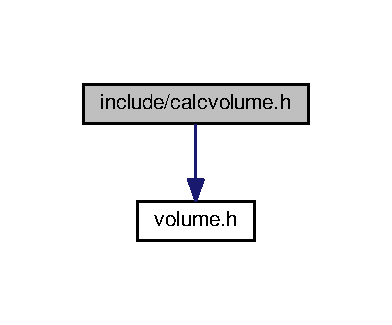
\includegraphics[width=188pt]{calcvolume_8h__incl}
\end{center}
\end{figure}
This graph shows which files directly or indirectly include this file\+:
\nopagebreak
\begin{figure}[H]
\begin{center}
\leavevmode
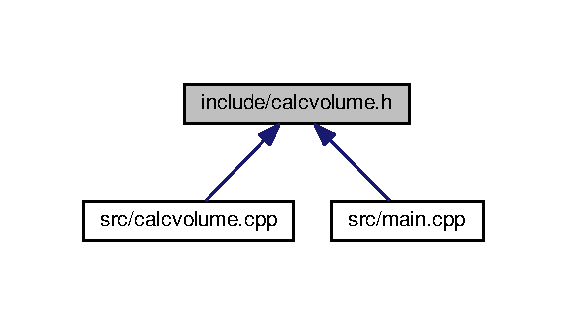
\includegraphics[width=272pt]{calcvolume_8h__dep__incl}
\end{center}
\end{figure}
\subsection*{Functions}
\begin{DoxyCompactItemize}
\item 
void \hyperlink{calcvolume_8h_aa5acf0ff0f4eb8061d1b86334d2838de}{calc\+Volume\+Piramide} (float \&base, float \&altura)
\begin{DoxyCompactList}\small\item\em Função que imprime o valor do volume da piramide. \end{DoxyCompactList}\item 
void \hyperlink{calcvolume_8h_af35d29634faa808e187b6635ac6e1fb9}{calc\+Volume\+Cubo} (float \&aresta)
\begin{DoxyCompactList}\small\item\em Função que imprime o valor do volume do cubo. \end{DoxyCompactList}\item 
void \hyperlink{calcvolume_8h_a994d3c26012b734a4cbabf0ce0c7b75b}{calc\+Volume\+Paralelepipedo} (float \&aresta1, float \&aresta2, float \&aresta3)
\begin{DoxyCompactList}\small\item\em Função que imprime o valor do volume do paralelepípedo. \end{DoxyCompactList}\item 
void \hyperlink{calcvolume_8h_addef3fdcde1a2b12007610961caffae5}{calc\+Volume\+Esfera} (float \&raio)
\begin{DoxyCompactList}\small\item\em Função que imprime o valor do volume da esfera. \end{DoxyCompactList}\end{DoxyCompactItemize}


\subsection{Detailed Description}
Arquivo cabeçalho contendo a definição das funções que solicitam ao usuário os dados necessários para o cálculo do volume com a figura geométrica e chamam as funções que realizam essa operação. 

\begin{DoxyAuthor}{Author}
Gabriel Barbosa (\href{mailto:gbsbarbosa.gb@gmail.com}{\tt gbsbarbosa.\+gb@gmail.\+com}) 

Ariel Oliveira (\href{mailto:ariel.oliveira01@gmail.com}{\tt ariel.\+oliveira01@gmail.\+com}) 
\end{DoxyAuthor}
\begin{DoxySince}{Since}
09/03/2017 
\end{DoxySince}
\begin{DoxyDate}{Date}
12/03/2017 
\end{DoxyDate}
\begin{DoxySeeAlso}{See also}
\hyperlink{volume_8h}{volume.\+h} 
\end{DoxySeeAlso}


\subsection{Function Documentation}
\index{calcvolume.\+h@{calcvolume.\+h}!calc\+Volume\+Cubo@{calc\+Volume\+Cubo}}
\index{calc\+Volume\+Cubo@{calc\+Volume\+Cubo}!calcvolume.\+h@{calcvolume.\+h}}
\subsubsection[{\texorpdfstring{calc\+Volume\+Cubo(float \&aresta)}{calcVolumeCubo(float &aresta)}}]{\setlength{\rightskip}{0pt plus 5cm}void calc\+Volume\+Cubo (
\begin{DoxyParamCaption}
\item[{float \&}]{aresta}
\end{DoxyParamCaption}
)}\hypertarget{calcvolume_8h_af35d29634faa808e187b6635ac6e1fb9}{}\label{calcvolume_8h_af35d29634faa808e187b6635ac6e1fb9}


Função que imprime o valor do volume do cubo. 


\begin{DoxyParams}{Parameters}
{\em aresta} & A\+R\+E\+S\+TA valor da aresta do cubo \\
\hline
\end{DoxyParams}
\index{calcvolume.\+h@{calcvolume.\+h}!calc\+Volume\+Esfera@{calc\+Volume\+Esfera}}
\index{calc\+Volume\+Esfera@{calc\+Volume\+Esfera}!calcvolume.\+h@{calcvolume.\+h}}
\subsubsection[{\texorpdfstring{calc\+Volume\+Esfera(float \&raio)}{calcVolumeEsfera(float &raio)}}]{\setlength{\rightskip}{0pt plus 5cm}void calc\+Volume\+Esfera (
\begin{DoxyParamCaption}
\item[{float \&}]{raio}
\end{DoxyParamCaption}
)}\hypertarget{calcvolume_8h_addef3fdcde1a2b12007610961caffae5}{}\label{calcvolume_8h_addef3fdcde1a2b12007610961caffae5}


Função que imprime o valor do volume da esfera. 


\begin{DoxyParams}{Parameters}
{\em raio} & R\+A\+IO valor do raio do cubo \\
\hline
\end{DoxyParams}
\index{calcvolume.\+h@{calcvolume.\+h}!calc\+Volume\+Paralelepipedo@{calc\+Volume\+Paralelepipedo}}
\index{calc\+Volume\+Paralelepipedo@{calc\+Volume\+Paralelepipedo}!calcvolume.\+h@{calcvolume.\+h}}
\subsubsection[{\texorpdfstring{calc\+Volume\+Paralelepipedo(float \&aresta1, float \&aresta2, float \&aresta3)}{calcVolumeParalelepipedo(float &aresta1, float &aresta2, float &aresta3)}}]{\setlength{\rightskip}{0pt plus 5cm}void calc\+Volume\+Paralelepipedo (
\begin{DoxyParamCaption}
\item[{float \&}]{aresta1, }
\item[{float \&}]{aresta2, }
\item[{float \&}]{aresta3}
\end{DoxyParamCaption}
)}\hypertarget{calcvolume_8h_a994d3c26012b734a4cbabf0ce0c7b75b}{}\label{calcvolume_8h_a994d3c26012b734a4cbabf0ce0c7b75b}


Função que imprime o valor do volume do paralelepípedo. 


\begin{DoxyParams}{Parameters}
{\em aresta1} & A\+R\+E\+S\+T\+A1 valor da aresta \#1 do paralelepípedo \\
\hline
{\em aresta2} & A\+R\+E\+S\+T\+A2 valor da aresta \#2 do paralelepípedo \\
\hline
{\em aresta3} & A\+R\+E\+S\+T\+A3 valor da aresta \#3 do paralelepípedo \\
\hline
\end{DoxyParams}
\index{calcvolume.\+h@{calcvolume.\+h}!calc\+Volume\+Piramide@{calc\+Volume\+Piramide}}
\index{calc\+Volume\+Piramide@{calc\+Volume\+Piramide}!calcvolume.\+h@{calcvolume.\+h}}
\subsubsection[{\texorpdfstring{calc\+Volume\+Piramide(float \&base, float \&altura)}{calcVolumePiramide(float &base, float &altura)}}]{\setlength{\rightskip}{0pt plus 5cm}void calc\+Volume\+Piramide (
\begin{DoxyParamCaption}
\item[{float \&}]{base, }
\item[{float \&}]{altura}
\end{DoxyParamCaption}
)}\hypertarget{calcvolume_8h_aa5acf0ff0f4eb8061d1b86334d2838de}{}\label{calcvolume_8h_aa5acf0ff0f4eb8061d1b86334d2838de}


Função que imprime o valor do volume da piramide. 


\begin{DoxyParams}{Parameters}
{\em base} & B\+A\+SE valor da base da piramide \\
\hline
{\em altura} & A\+L\+T\+U\+RA valor da altura da piramide\\
\hline
{\em base} & B\+A\+SE valor da base da piramide \\
\hline
{\em altura} & A\+L\+T\+U\+RA valor da altura da piramide Funcao que imprime o valor do volume da piramide \\
\hline
{\em base} & B\+A\+SE valor da base da piramide \\
\hline
{\em altura} & A\+L\+T\+U\+RA valor da altura da piramide \\
\hline
\end{DoxyParams}

\hypertarget{volume_8h}{}\section{Referência do Arquivo include/questao\+\_\+1/volume.h}
\label{volume_8h}\index{include/questao\+\_\+1/volume.\+h@{include/questao\+\_\+1/volume.\+h}}


Arquivo cabeçalho contendo a definição das funções que calculam o volume de figuras geométricas espaciais.  


Este grafo mostra quais arquivos estão direta ou indiretamente relacionados com este arquivo\+:
\nopagebreak
\begin{figure}[H]
\begin{center}
\leavevmode
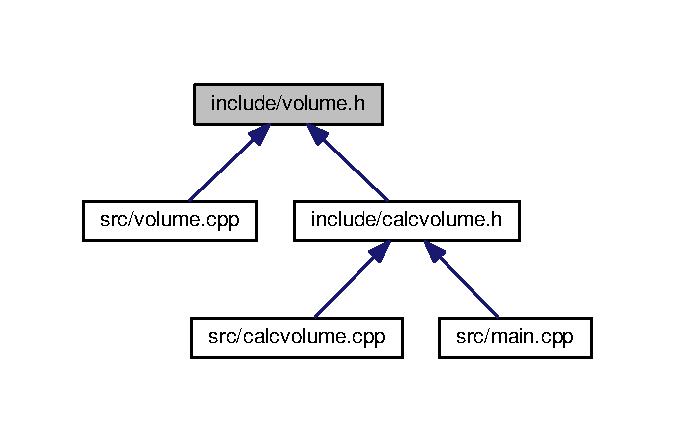
\includegraphics[width=350pt]{volume_8h__dep__incl}
\end{center}
\end{figure}
\subsection*{Funções}
\begin{DoxyCompactItemize}
\item 
float \hyperlink{group__Calc__Volume_ga4a36098bad980501fa8e5d0229309098}{volume\+Piramide} (float \&base, float \&altura)
\begin{DoxyCompactList}\small\item\em Função que calcula o valor do volume da pirâmide. \end{DoxyCompactList}\item 
float \hyperlink{group__Calc__Volume_ga43aaef1a010e2ccbe7e5389aa5be3366}{volume\+Cubo} (float \&aresta)
\begin{DoxyCompactList}\small\item\em Função que calcula o valor do volume do cubo. \end{DoxyCompactList}\item 
float \hyperlink{group__Calc__Volume_gadf67b3277ecfcf3e6e225e1f66e30a23}{volume\+Paralelepipedo} (float \&aresta1, float \&aresta2, float \&aresta3)
\begin{DoxyCompactList}\small\item\em Função que calcula o valor do volume do paralelepípedo. \end{DoxyCompactList}\item 
float \hyperlink{group__Calc__Volume_gaf649387c42d43094c7c81e2f26face42}{volume\+Esfera} (float \&raio)
\begin{DoxyCompactList}\small\item\em Função que calcula o valor do volume da esfera. \end{DoxyCompactList}\end{DoxyCompactItemize}


\subsection{Descrição Detalhada}
Arquivo cabeçalho contendo a definição das funções que calculam o volume de figuras geométricas espaciais. 

\begin{DoxyAuthor}{Autor}
Ariel Oliveira (\href{mailto:ariel.oliveira01@gmail.com}{\tt ariel.\+oliveira01@gmail.\+com}) 
\end{DoxyAuthor}
\begin{DoxySince}{Desde}
10/08/2017 
\end{DoxySince}
\begin{DoxyDate}{Data}
15/08/2017 
\end{DoxyDate}

\hypertarget{calcvolume_8cpp}{}\section{Referência do Arquivo src/calcvolume.cpp}
\label{calcvolume_8cpp}\index{src/calcvolume.\+cpp@{src/calcvolume.\+cpp}}


Arquivo de corpo contendo a implementação das funções que solicitam ao usuário os dados necessários para o cálculo do volume com a figura geométrica e chamam as funções que realizam essa operação.  


{\ttfamily \#include $<$iostream$>$}\\*
{\ttfamily \#include \char`\"{}calcvolume.\+h\char`\"{}}\\*
Gráfico de dependência de inclusões para calcvolume.\+cpp\+:
\nopagebreak
\begin{figure}[H]
\begin{center}
\leavevmode
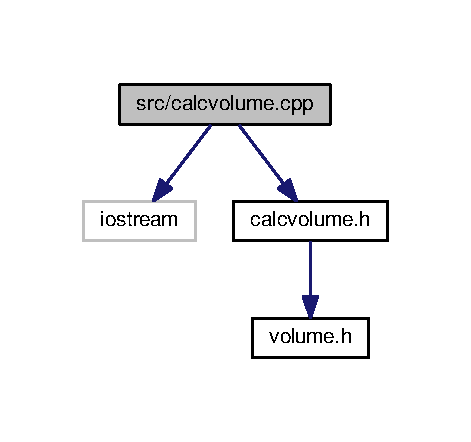
\includegraphics[width=226pt]{calcvolume_8cpp__incl}
\end{center}
\end{figure}
\subsection*{Funções}
\begin{DoxyCompactItemize}
\item 
void \hyperlink{group__Figuras__Espaciais__Imprime__Volume_gaa5acf0ff0f4eb8061d1b86334d2838de}{calc\+Volume\+Piramide} (float \&base, float \&altura)
\begin{DoxyCompactList}\small\item\em Função que imprime o valor do volume da pirâmide. \end{DoxyCompactList}\item 
void \hyperlink{group__Figuras__Espaciais__Imprime__Volume_gaf35d29634faa808e187b6635ac6e1fb9}{calc\+Volume\+Cubo} (float \&aresta)
\begin{DoxyCompactList}\small\item\em Função que imprime o valor do volume do cubo. \end{DoxyCompactList}\item 
void \hyperlink{group__Figuras__Espaciais__Imprime__Volume_ga994d3c26012b734a4cbabf0ce0c7b75b}{calc\+Volume\+Paralelepipedo} (float \&aresta1, float \&aresta2, float \&aresta3)
\begin{DoxyCompactList}\small\item\em Função que imprime o valor do volume do paralelepípedo. \end{DoxyCompactList}\item 
void \hyperlink{group__Figuras__Espaciais__Imprime__Volume_gaddef3fdcde1a2b12007610961caffae5}{calc\+Volume\+Esfera} (float \&raio)
\begin{DoxyCompactList}\small\item\em Função que imprime o valor do volume da esfera. \end{DoxyCompactList}\end{DoxyCompactItemize}


\subsection{Descrição Detalhada}
Arquivo de corpo contendo a implementação das funções que solicitam ao usuário os dados necessários para o cálculo do volume com a figura geométrica e chamam as funções que realizam essa operação. 

\begin{DoxyAuthor}{Autor}
Gabriel Barbosa (\href{mailto:gbsbarbosa.gb@gmail.com}{\tt gbsbarbosa.\+gb@gmail.\+com}) 

Ariel Oliveira (\href{mailto:ariel.oliveira01@gmail.com}{\tt ariel.\+oliveira01@gmail.\+com}) 
\end{DoxyAuthor}
\begin{DoxySince}{Desde}
09/03/2017 
\end{DoxySince}
\begin{DoxyDate}{Data}
12/03/2017 
\end{DoxyDate}
\begin{DoxySeeAlso}{Veja também}
\hyperlink{calcvolume_8h}{calcvolume.\+h} 
\end{DoxySeeAlso}

\hypertarget{main_8cpp}{}\section{src/main.cpp File Reference}
\label{main_8cpp}\index{src/main.\+cpp@{src/main.\+cpp}}


Programa que cálcula área, perímetro e volume de figuras geométricas planas e espaciais.  


{\ttfamily \#include $<$iostream$>$}\\*
{\ttfamily \#include $<$limits$>$}\\*
{\ttfamily \#include \char`\"{}calcarea.\+h\char`\"{}}\\*
{\ttfamily \#include \char`\"{}calcvolume.\+h\char`\"{}}\\*
{\ttfamily \#include \char`\"{}calcperimetro.\+h\char`\"{}}\\*
Include dependency graph for main.\+cpp\+:
% FIG 0
\subsection*{Functions}
\begin{DoxyCompactItemize}
\item 
void {\bfseries triangulo} ()\hypertarget{main_8cpp_a8928cef04d4cd48e92adf3569f6d185b}{}\label{main_8cpp_a8928cef04d4cd48e92adf3569f6d185b}

\item 
void {\bfseries retangulo} ()\hypertarget{main_8cpp_afa7da114af5845aed90385aaad07745f}{}\label{main_8cpp_afa7da114af5845aed90385aaad07745f}

\item 
void {\bfseries quadrado} ()\hypertarget{main_8cpp_a59a769deb5a89245b0b2a7760179708e}{}\label{main_8cpp_a59a769deb5a89245b0b2a7760179708e}

\item 
void {\bfseries circulo} ()\hypertarget{main_8cpp_a28482bc381ce414df86e4fdb9e3e6da5}{}\label{main_8cpp_a28482bc381ce414df86e4fdb9e3e6da5}

\item 
void {\bfseries piramide} ()\hypertarget{main_8cpp_ae3945922f925bc3d1fd95c5dc4ff6987}{}\label{main_8cpp_ae3945922f925bc3d1fd95c5dc4ff6987}

\item 
void {\bfseries cubo} ()\hypertarget{main_8cpp_af0b7d023166ce6902197d4082a66ad03}{}\label{main_8cpp_af0b7d023166ce6902197d4082a66ad03}

\item 
void {\bfseries paralelepipedo} ()\hypertarget{main_8cpp_af5c3350f35c2d9ae97c0243b7aeac39e}{}\label{main_8cpp_af5c3350f35c2d9ae97c0243b7aeac39e}

\item 
void {\bfseries esfera} ()\hypertarget{main_8cpp_a947bf2f326598c591bbdbf77a0280266}{}\label{main_8cpp_a947bf2f326598c591bbdbf77a0280266}

\item 
void {\bfseries menu} ()\hypertarget{main_8cpp_a2a0e843767aeea4f433a28b9c54f573a}{}\label{main_8cpp_a2a0e843767aeea4f433a28b9c54f573a}

\item 
void {\bfseries continua} (char $\ast$s)\hypertarget{main_8cpp_a5b6e29af98c7595c8ddf9771382fd141}{}\label{main_8cpp_a5b6e29af98c7595c8ddf9771382fd141}

\item 
void {\bfseries menu\+Escolha} (int escolha)\hypertarget{main_8cpp_a880038c883d20b974c3972ca68b2bdb0}{}\label{main_8cpp_a880038c883d20b974c3972ca68b2bdb0}

\item 
int {\bfseries main} ()\hypertarget{main_8cpp_ae66f6b31b5ad750f1fe042a706a4e3d4}{}\label{main_8cpp_ae66f6b31b5ad750f1fe042a706a4e3d4}

\end{DoxyCompactItemize}


\subsection{Detailed Description}
Programa que cálcula área, perímetro e volume de figuras geométricas planas e espaciais. 

Figuras geométricas planas possuem apenas área e perímetro, assim como as espaciais não possuem perímetro \begin{DoxyAuthor}{Author}
Gabriel Barbosa (\href{mailto:gbsbarbosa.gb@gmail.com}{\tt gbsbarbosa.\+gb@gmail.\+com}) 

Ariel Oliveira (\href{mailto:ariel.oliveira01@gmail.com}{\tt ariel.\+oliveira01@gmail.\+com}) 
\end{DoxyAuthor}
\begin{DoxySince}{Since}
09/03/2017 
\end{DoxySince}
\begin{DoxyDate}{Date}
12/03/2017 
\end{DoxyDate}

%--- End generated contents ---

% Index
\backmatter
\newpage
\phantomsection
\clearemptydoublepage
\addcontentsline{toc}{chapter}{Index}
\printindex

\end{document}
